\documentclass{arabicClass}

\begin{document}
	\renewcommand{\jot}{7pt}
	\abovedisplayskip=7pt
	\belowdisplayskip=7pt
	
	\renewcommand{\theequation}{\arabic{equation}.\arabic{chapter}}
	
	\newgeometry{
	margin=0.5in
}
\begin{titlepage}
	\begin{minipage}{0.2\textwidth}
		\raggedleft\includegraphics[scale=0.2]{Title Page/university.png}
	\end{minipage}
	\hfill
	\begin{minipage}{0.5\textwidth}
		\centering
		% \large
		\textbf{وزارة التعليم العالي والبحث العلمي}\\
		\textbf{جامعة البصرة}\\
		\textbf{كلية التربية للعلوم الصرفة}\\
		\textbf{قسم الرياضيات - للدراسة المسائية}
	\end{minipage}
	\hfill
	\begin{minipage}{0.2\textwidth}
		\raggedright\includegraphics[scale=0.16]{Title Page/college.png}   
	\end{minipage}
	
	\vspace{1cm}
	
	\begin{center}
		\large \textbf{\textcolor{red}{حل المعادلات التفاضلية الاعتيادية بمتسلسلات القوى}}\\
		\large \textbf{\LR{\textcolor{red}{Solving Ordinary Differential Equations by Power Series}}}
	\end{center}
	\vfill
	
	\begin{center}
		\large
		\textbf{بحث تخرج تقدم به الى}
	\end{center}
	
	\begin{center}
		\large
		\textbf{قسم الرياضيات كلية التربية للعلوم الصرفة جامعة البصرة\\
			\vspace{6pt}
			وهو جزء من متطلبات نيل شهادة بكالوريوس علوم الرياضيات}
	\end{center}
	\vfill
	\begin{center}
		\large
		\textbf{من قبل الطالبة}\\
		\vspace{8pt}
		\large
		\textbf{منى وليد عباس}
	\end{center}
	\vspace{10pt}
	\begin{center}
		\large
		\textbf{إشراف}\\
		\vspace{8pt}
		\large
		\textbf{م. د. مهند موسى عيسى}
	\end{center}
	\vspace{80pt}
	\begingroup
	\large{\raggedleft \textbf{2025 م}} {\hfill \textbf{1446 هــ}}
	\endgroup
\end{titlepage}
\restoregeometry
	\pagenumbering{roman}
	\amirifont
	\chapter*{الآية}

\begin{Large}
	\textbf{قال تعالى}
	\begin{center}
(وَلَسَوْفَ يُعْطِيكَ رَبُّكَ فَتَرْضَى)
	\end{center}
	\begin{flushleft}
		\textbf{صدق الله العلي العظيم}\\
		\noindent
		\textbf{سورة الضحى (5)}
	\end{flushleft}
	
\end{Large}



	\chapter*{الاهداء}
\addcontentsline{toc}{chapter*}{الاهداء}

\begin{doublespacing}
	\begin{center}
إلى من كانوا ولا يزالون مصدر إلهامي ودعمي في كل خطوة، أهدى هذا البحث:

إلى والديّ العزيزين، اللذين كانا وما زالا الركيزة الأساسية في حياتي، فبفضلهما وعطائهما اللامحدود، تعلمت كيف أواجه تحديات الحياة بثقة وأمل. 
إلى أخوتي الأحباء، الذين كانوا دائمًا إلى جانبي، يقدمون لي النصائح والمساعدة ويشجعونني على السعي نحو الأفضل.
إلى أصدقائي الأعزاء، الذين لم يبخلوا بتقديم الدعم والمساندة في كل مرحلة من مراحل هذا البحث، وكانوا خير رفقاء في درب العلم والمثابرة.

أقدم هذا العمل عربون شكر وامتنان لكم جميعًا، فبدونكم لم يكن لي أن أحقق هذا الإنجاز.
\end{center}
\end{doublespacing}

	\chapter*{شكر و تقدير}
الحمد لله الذي وفقني لإتمام هذا البحث وأعانني على تجاوز جميع التحديات، والصلاة والسلام على سيدنا محمد وعلى آله اجمعين.\\ \\ 
أتوجه بخالص الشكر والتقدير إلى أساتذتي الأفاضل على دعمهم وتوجيهاتهم القيمة طوال مسيرتي الدراسية، وعلى رأسهم \textbf{الأستاذ المشرف مرتضئ جاسم محمد }الذي كان خير معين لي في إتمام هذا البحث. فله الفضل بعد الله في توجيه مساري البحثي، ولم يبخل عليّ بالنصح والتوجيه .كما أشكر كل من علمني حرفا في حياتي الدراسية، وأخص منهم كل من درسني الرياضيات يوما، سواء في الصفوف المدرسية أو لآحقاً عندما تخصصت الرياضيات في جامعة البصرة\\ \\ 
وأخيرًا، أوجه شكري لكل من ساهم بشكلٍ مباشر أو غير مباشر في إنجاز هذا البحث، سائلًا الله أن جعل هذا العمل خالصًا لوجهه الكريم، وأن ينفع به الجميع
   \arabicfont
	\tableofcontents
   \clearpage
   \pagenumbering{arabic}	
	\chapter*{الملخص}
\addcontentsline{toc}{chapter*}{الملخص}

تناول هذا البحث أهم الاختبارات اللّا معلمية 
\LR{(Non-parametric Tests)}، التي تُعد من الأدوات الإحصائية الأساسية عند عدم تحقق الافتراضات المطلوبة في الاختبارات المعلمية، كعدم توفر التوزيع الطبيعي أو تجانس التباين. وقد تطرق البحث إلى تعريف الاختبارات اللا معلمية، وبيان الفرق بينها وبين الاختبارات المعلمية من حيث الشروط والمرونة في التطبيق، مع توضيح مميزاتها وعيوبها.

كما شمل البحث عرضًا لأبرز الاختبارات اللا معلمية المستخدمة في تحليل البيانات، مثل اختبار مان-ويتني 
\LR{(Mann-Whitney U Test)} للمجموعات المستقلة، واختبار ويلكوكسون \LR{(Wilcoxon Signed-Rank Test)} للبيانات المرتبطة وغيرها من الاختبارات الشائعة. وتم توضيح استخدامات كل اختبار، وخطوات تطبيقه، وكيفية تفسير نتائجه.

واختُتم البحث بالتأكيد على أهمية هذه الاختبارات في مجالات متعددة، خصوصًا في البحوث التي تتعامل مع بيانات رتبية أو ذات توزيع غير طبيعي، مما يجعلها أدوات فعالة في دعم القرارات الإحصائية عندما تكون الشروط المعلمية غير متحققة.
	\chapter*{مقدمة}
\addcontentsline{toc}{chapter*}{مقدمة}

​تحويل لابلاس هو أداة رياضية قوية تُستخدم لتحويل المعادلات التفاضلية، خاصة الخطية ذات المعاملات الثابتة، إلى معادلات جبرية أبسط في مجال التردد المركب. يُسهّل هذا التحويل عملية الحل، خصوصًا عندما تكون المعادلة مصحوبة بشروط ابتدائية، حيث يتم دمج هذه الشروط مباشرة في المعادلة المحوّلة، مما يلغي الحاجة إلى حساب الثوابت بشكل منفصل كما في الطرق التقليدية.​[5]

\noindent
يُستخدم تحويل لابلاس على نطاق واسع في مجالات متعددة مثل الهندسة الكهربائية لتحليل الدوائر الكهربائية، والهندسة الميكانيكية لدراسة الاهتزازات، وفي أنظمة التحكم لتحليل استجابات الأنظمة. بعد حل المعادلة الجبرية في مجال التردد، يتم استخدام تحويل لابلاس العكسي للعودة إلى الحل في المجال الزمني، مما يوفر فهمًا دقيقًا لسلوك النظام الأصلي.​[3]

\noindent
بفضل قدرته على تبسيط المعادلات المعقدة والتعامل مع الشروط الابتدائية بفعالية، يُعد تحويل لابلاس أداة لا غنى عنها في تحليل الأنظمة الديناميكية وحل المعادلات التفاضلية في مختلف التخصصات العلمية والهندسية.[2]
	
	\chapter{مفاهيم أساسية}

\section[المعادلة التفاضلية الاعتيادية]{المعادلة التفاضلية الاعتيادية \cite{ode}}
هي علاقة بين المتغير المعتمد ومتغير مستقل واحد وتدخل فيها المشتقات او التفاضلات. الصيغة العامة للمعادلة التفاضلية الاعتيادية
\begin{equation}
	F(x, y, y', y'', \dots) = 0
\end{equation}
حيث $y$ المتغير المعتمد و $x$ المتغير المستقل و $F$ اي دالة. الان سوف نعطي بعض الامثلة على المعادلات التفاضلية الاعتيادية
\begin{align}
	\frac{dy}{dx} + y &= 3x^2\\[5pt]
	x\frac{d^3 y}{dx^3} + (2\sin x)\frac{d^2 y}{dx^2}\frac{dy}{dx} &= (3-x^2)y\\[5pt]
	\frac{d^2 y}{dx^2} + \frac{1}{x}\, \frac{dy}{dx} + y &=0 \\[5pt]
	(x-y)dx + (x+y)dy &= 0
\end{align}

\section[تصنيف المعادلات التفاضلية الاعتيادية]{تصنيف المعادلات التفاضلية الاعتيادية \cite{ode}}

سوف نصنف المعادلات التفاضلية الاعتيادية حسب الاتي
\subsection*{1. رتبة المعادلات التفاضلية الاعتيادية}
اذا كانت المشتقة النونية $y^{(n)}$ هي اعلى مشتقة تظهر بالمعادلة التفاضلية الاعتيادية قيل أن هذه المعادلة من الرتبة $n$.\\
\textbf{مثال:} لدينا المعادلات (2) و (5) معادلات تفاضلية من الرتبة الاولى. اما المعادلة (2) هي من الرتبة الثانية و المعادلة (4) من الرتبة الثالثة.

\subsection*{2. درجة المعادلة التفاضلية الاعتيادية}
هي الاس المرفوع اليها اعلى مشتقة تظهر بالمعادلة التفاضلية. وقبل تحديد درجة المعادلة يجب وضعها على صورة قياسية وصحيحة من حيث المشتقات.\\
\textbf{مثال:} المعادلات من (2) الى (5) كلها من الدرجة الاولى اما المعادلة
\begin{equation}
	\left(\frac{d^2 y}{dx^2}\right)^3 + x\left(\frac{dy}{dx}\right) + x^2 y^2 = e^x \sin x
\end{equation}
فهي معادلية تفاضلية من الرتبة الثانية و الدرجة الثالثة.

\subsection*{3. المعادلة التفاضلية الخطية}
هي المعادلة التفاضلية التي تكون خطية في المتغير المعتمد ومشتقاته جميعاً\\
\textbf{مثال:} المعادلة
\begin{equation}
	x^2y'' + xy' + x^2 y = \sin x
\end{equation}
هي معادلة خطية من الرتبة الثانية حيث ان كلاً من المتغير المعتمد $y$ ومشتقاته $y', y''$ خطية

اذا لم تكن المعادلية التفاضلية خطية فانها معادلة تفاضلية لا خطية\\
\textbf{مثال:} المعادلات التفاضلية التالية غير خطية
\begin{align}
	yy'' + y' &=0\\[5pt]
	y' + x\sqrt{y} &= \sin x\\[5pt]
	y''' + x^2 y'' + \sin y &= 0
\end{align}

\subsection*{4. المعادلة التفاضلية الاعتيادية الخطية المتجانسة}
تكون على الصيغة
\begin{equation}
	P_n(x) y^{(n)} + P_{n-1}(x) y^{(n-1)}+ \cdots + P_1(x) y' + P_0(x) y = 0
\end{equation}
\textbf{مثال:} المعادلة
\begin{equation}
	x^2 y'' + xy' + (x^2 - 1) y =0
\end{equation}
معادلة تفاضلية اعتيادية خطية متجانسة من الرتبة الثانية.

\setcounter{equation}{0}
\section[المعادلة التفاضلية الجزئية]{المعادلة التفاضلية الجزئية \cite{pde1}}
المعادلة التفاضلية الجزئية هي معادلة تتضمن متغير معتمد ذات متغيرين او اكثر ، والمشتقات الجزئية لهذه بالنسبة الى بعض تلك المتغيرات او كلها\\ [5pt]
الصيغة العامة للمعادلة التفاضلية الجزئية هي 
\begin{equation}
	F(x,y,z,t,\dots,u_x, u_y, u_z, u_t, \dots) = 0
\end{equation}
حيث $u$ هو المتغير المعتمد و $x,y,z,t,\dots$ هي المتغيرات المستقلة.\\[5pt]
\textbf{مثال:} كل مما يأتي معادلة تفاضلية جزئية
\begin{align}
	&\frac{\partial u}{\partial x} = t\\[5pt]
	&x\frac{\partial u}{\partial x} - t\frac{\partial u}{\partial t} = 4\\[5pt]
	&(x^2 + t^2)\frac{\partial^2 u}{\partial x\partial t} - 3\frac{\partial u}{\partial x} + x\left(\frac{\partial u}{\partial t}\right)^4 = e^x\\[5pt]
	&x\left(\frac{\partial u}{\partial x}\right)^3 - y\left(\frac{\partial^3 u}{\partial x\partial t^2}\right)^2 = 6x\frac{\partial u}{\partial x} \frac{\partial u}{\partial t}
\end{align}

\section[تصنيف المعادلات التفاضلية الجزئية]{تصنيف المعادلات التفاضلية الجزئية\cite{pde1}}
كما الحال في المعادلات التفاضلية الاعتيادية سوف نصنف المعادلات التفاضلية الجزئية كالآتي

\subsection*{1. رتبة ودرجة المعادلة التفاضلية}
كما في حالة المعادلات التفاضلية الاعتيادية تعرف رتبة المعادلة التفاضلية الجزئية بانها اعلى مشتقة فيها كما ان درجة المعادلة التفاضلية الجزئية هي اس اعلى مشتقة فيها بشرط ان يكون عدداً صحيحاً غير سالب.\\ [5pt]
\textbf{مثال:} المعادلتان (2) و (3) في المثال اعلاه من الرتبة الاولى و الدرجة الاولى والمعادلة (4) من الرتبة الثانية والدرجة الاولى والمعادلة (5) من الرتبة الثالثة والدرجة الثانية

\subsection*{2. المعادلة التفاضلية الجزئية الخطية}
تسمى المعادلة التفاضلية الجزئية خطية اذا كان مجموع اسس المتغير المعتمد ومشتقاته في كل من حدوده لا يزيد على (1) بشرط ان تكون الاسس اعداداً صحيحة غير سالبة وعلى سبيل المثال فإن المعادلة:
\begin{equation*}
	(x-t) \frac{\partial^3 u}{\partial x^3} + 4x \frac{\partial^3 u}{\partial x\partial t^2} - \frac{\partial ^2 u}{\partial x^2} + t \frac{\partial u}{\partial t} + tu = e^x
\end{equation*}
خطية، ولكن المعادلات
\begin{align*}
	& u \frac{\partial^2  u}{\partial x^2} - 4x \frac{\partial^2 u}{\partial x\partial y} = 0\\[5pt]
	&\left(\frac{\partial u}{\partial x}\right)^2 - 5xu = 0
\end{align*}
غير خطية

\subsection*{3. المعادلة التفاضلية الجزئية الخطية المتجانسة}
تسمى المعادلة التفاضلية الجزئية الخطية متجانسة اذا كانت كل المشتقات الجزئية فيها متساوية في الرتبة.\\
وعلى سبيل المثال فإن المعادلتين الاتيتين
\begin{align*}
&u_{xx} - x u_{tx} = 4x^2\\
&x^2 u_{xxx} + 5xt u_{txx} - u_{xxx} = x^2 + t^2
\end{align*}
متجانستين، ولكن المعادلتين
\begin{align*}
	&x^2 u_{xxx} + 5xt u_{txx} + u_{xx} = x^2\\
	&u_x + xu = t
\end{align*}
غير متجانستين

\section[عدد المتغيرات و الانماط الثلاث الاساسية]{عدد المتغيرات و الانماط الثلاث الاساسية \cite{pde3}}
سوف نهتم بدراسة المعادلات التفاضلية الجزئية بمتغيرين مستقلين والتي تأخذ الشكل العام
\begin{equation}
	a u_{xx} + 2bu_{tx} + cu_{tt} + du_x + eu_t + fu + g = 0
\end{equation}
حيث $a,b,c,d,e,f$ دوال للمتغيرين $x,t$. سوف ندرس المعادلة (6) من خلال المقدار المميز
\begin{equation}
	\Delta = b^2 - 4ac
\end{equation}

\subsection*{1. المعادلة التفاضلية الجزئية المكافئية}
تكون المعادلة (6) مكافئية اذا كان $\Delta =0 $ \\
\textbf{مثال:}
 \begin{equation*}
 	u_{xx} - u_y = 0
 \end{equation*}
 
 \subsection*{2. المعادلة التفاضلية الجزئية الناقصية}
 تكون المعادلة (6) ناقصية اذا كان $\Delta < 0 $ \\
 \textbf{مثال:}
 \begin{equation*}
 	u_{xx} + u_{yy} = 0
 \end{equation*}
 
 \subsection*{3. المعادلة التفاضلية الجزئية الزائدية}
 تكون المعادلة (6) زائدية اذا كان $\Delta > 0$ \\
 \textbf{مثال:}
 \begin{equation*}
 	u_{xx} - u_{yy} = 0
 \end{equation*}
 
 \section[الشروط الابتدائية و الشروط الحدودية]{الشروط الابتدائية والشروط الحدودية \cite{pde2}}
 
 \subsection*{1. الشرط الابتدائي}
 يتم تفسير احد المتغيرات المستقلة على انه الزمن $t$. و نفرض الشروط عند لحظة معينة. على سبيل المثال
 $u(x, t_0) = u_0(x)$
 
 \subsection*{2. الشرط الحدودي}
 نفرض الشروط على حدود المجال $\Omega$. على سبيل المثال
 $u|_{\partial \Omega} = \phi$
 حيث $\partial\Omega$ هي حدود المجال $\Omega$.
 
 
	\chapter{تطبيقات}

\section{معادلة الحركة \en{Equation of Motion}}

من قانون نيوتن الثاني لحركة جسم ما 
\begin{equation}
	\label{eq:newton2law}
	\sum \vec{F} = m a
\end{equation}
حيث 
\begin{itemize}
	\item $\sum \vec{F}$ مجموع القوى المؤثرة على الجسم.
	\item $m$ كتلة الجسم.
	\item $a$ تسارع الجسم ($a = \dfrac{d^2 y}{dt^2}$)
\end{itemize}

\begin{english}
	\begin{figure}[ht]
	\centering
	\includegraphics[width=0.3\textwidth]{Figures/em.jpg}
	\caption{Equation of motion}
\end{figure}
\end{english}

نطبق هذه المعادلة على سقوط حر لجسم (نهمل قوة مقاومة الهواء) اذن هناك قوة واحدة تؤثر على الجسم وهي (وزن الجسم). يمكن حساب وزن الجسم من خلال القانون 
\[
\vec{F}_w = - mg
\]
حيث $g$ تعجيل الجاذبية الارضي. اذن بالتعويض في \eqref{eq:newton2law} نحصل على 
\begin{equation}
	\label{eq:freefall}
	- mg = m \frac{d^2 y}{dt^2} \Rightarrow \frac{d^2 y}{dt^2}  = -g
\end{equation}
مع الشروط الابتدائية
\begin{itemize}
	\item $y(0) = y_0$ موضع السقوط.
	\item $y'(0) = v_0$ السرعة الابتدائية.
\end{itemize}
الآن نطبق تحويل لابلاس على المعادلة وتعويض الشروط الابتدائية
\[
\LL\{y''\} = \LL\{-g\}
\]
\[
s^2Y(s) - s y(0) - y'(0) = \frac{-g}{s} 
\]
\[
Y(s) = \frac{1}{s^2} \left[\frac{-g}{s} + sy_0 + v_0\right]
\]
\[
Y(s) = \frac{-g}{s^3} + \frac{v_0}{s^2} + \frac{y_0}{s}
\]
بتطبيق لابلاس العكسي نحصل على
\begin{equation}
	\label{eq:motionsol}
	y(t) = -\frac{1}{2}gt^2 + v_0 t +y_0
\end{equation}
هذه المعادلة تصف موضع الجسم بعد مرور $t$ من السقوط.\\ \\
\noindent
\textbf{مثال عددي}\\
\noindent
سقط جسم من ارتفاع $y_0 = 100\text{m}$ بسرعة ابتدائية $v_0 = 0 $ المطلوب ايجاد الارتفاع بعد $t = 2\sec$
\begin{solution}
	تعجيل الجاذبية $g = 9.8 \text{m}/\sec^2$ اذن
	\[
	y(2) = -\frac{1}{2} \times 9.8 \times (2)^2 + 0 \times 2 + 100 = 80.4 \text{m}
	\]
\end{solution}

\section{معادلة تدفق بوازوي \en{Poiseuille's Flow Equation}}
يعد قانون بوازوي من القوانين الاساسية في ميكانيكا الموائع. حيث يصف تدفق الموائع اللزجة داخل الانابيب الدقيقة. لكي نشتق هذا القانون نستخدم من معادلات نافير ستوكس \\(\en{Navier Stokes Equations}) للحالة الخاصة بتدفق طبقي منتظم لسائل لزج داخل انبوب اسطواني افقي.\\
\noindent
\textbf{الفرضيات}
\begin{itemize}
	\item السريان ثابت (لا يوجد تغير زمني).
	\item السريان طبقي ومتناظر حول محور الانبوب.
	\item السائل غير قابل للانضغاط.
	\item لا توجد قوة خارجية (مثل الجاذبية) والضغط فقط هو المؤثر.
	\item السرعة تعتمد فقط على نصف القطر وليس على الطول $z$ او الزمن $t$.
\end{itemize}

\begin{english}
	\begin{figure}[ht]
		\centering
		\includegraphics[width=0.5\textwidth]{Figures/pe.jpg}
		\caption{Poiseuille's Flow}
	\end{figure}
\end{english}

\subsection*{معادلة نافير ستوكس المبسطة في الاتجاه \textit{z}}
نبدأ من معادلة نافير ستوكس العامة في الاتجاه $z$ 
\begin{equation}
	\label{eq:generalnavierstokes}
	\rho\left(
	\frac{\partial v_z}{\partial t} + \vec{v} \cdot \nabla v_z 
	\right)
	= - \frac{\partial p}{\partial z} + \mu \nabla^2 v_z
\end{equation}
لكن بالفرضيات التي ذكرناها تصبح المعادلة \eqref{eq:generalnavierstokes}:
\[
\frac{dp }{dz} = \mu \cdot \frac{1}{r} \frac{d}{dr} \left(r \frac{dv_z}{dr}\right)
\]
ولكن $dp/dz$ ثابت لأنه يعتمد فقط على $z$. والسريان غير متغير في $z$. نفرض
\[
\frac{dp}{dz} = \frac{- \Delta p}{L}
\]
حيث 
\begin{itemize}
	\item $\Delta p$ فرق الضغط.
	\item  $L$ طول الانبوب.
\end{itemize}
اذن تصبح المعادلة 
\begin{align}
	\frac{d}{dr} \left(r \frac{dv_z}{dr}\right) = \frac{-\Delta p}{\mu L} r \notag\\
		\label{eq:poiseuillflow}
		r \frac{d^2 v_z}{dr^2} + \frac{dv_z}{dr} =  \frac{-\Delta p}{\mu L} r 
\end{align}
مع الشروط الحدودية
\[
v_z(0) = \text{finite}, \quad v_z(R) = 0
\]
الآن نطبق تحويل لابلاس على \eqref{eq:poiseuillflow} نحصل على
\[
\LL\left\{r \frac{d^2 v_z}{dr^2} + \frac{dv_z}{dr}\right\} = \LL\left\{\frac{-\Delta p}{\mu L} r\right\}
\]
\[
-\frac{d}{ds} \left[s^2 V(s) - s v_z(0) - v_z'(0)\right] + \left[sV(s) - v_z(0)\right] =  \frac{-\Delta p}{\mu L s^2}
\]
\[
-s^2V'(s) -2s V(s) + v_z(0) + sV(s) - v_z(0) = \frac{-\Delta p}{\mu L s^2}
\]
\[
V'(s) + \frac{1}{s} V(s) = \frac{\Delta p}{\mu L s^4}
\]
بإستخدام عامل التكامل 
\[
I(s) = \exp\left(\int \frac{1}{s}\right) = \exp(\ln s) = s
\]
اذن يكون الحل
\[
I(s) V(s) = \int  \frac{\Delta p}{\mu L s^4} I(s)\, ds
\]
\[
s V(s) = \int \frac{\Delta p}{\mu L s^3} \, ds
\]
\[
s V(s) = -\frac{\Delta p}{2\mu L s^2} + C
\]
\[
V(s) = -\frac{\Delta p}{2\mu L s^3} + \frac{C}{s}
\]
بتطبيق لابلاس العكسي
\[
v_z(r) = - \frac{\Delta p}{4\mu L } r^2 + C
\]
بما ان $v_z(R) = 0 $
\[
C = \frac{\Delta p}{4\mu L } R^2
\]
اذن الحل النهائي
\[
v_z(r) = \frac{\Delta p}{4\mu L } (R^2 - r^2)
\]
الآن نستخرج معدل التدفق الحجمي $Q$ بالقانون
\begin{align*}
	Q &= \int_0^R v_z(r) \cdot 2\pi r \, dr\\
	&= \int_{0}^{R} \left(\frac{\Delta p}{4\mu L } (R^2 - r^2)\right)\cdot 2\pi r\, dr
\end{align*}

بالتكامل نحصل على 
\[
Q = \frac{\pi R^4 \Delta p}{8 \mu L}
\]
تسمى هذه المعادلة بقانون بوازوي.\\ \\
\noindent
\textbf{مثال تطبيقي}\\
\noindent
في الاوعية الدموية الصغيرة مثل الشرايين الدقيقة والشعيرات الدموية، يمكن اعتبار الدم كسائل لزج يتدفق تدفق طبقي. هنا نستخدم قانون بوازوي لتقدير معدل تدفق الدم عبر وعاء دموي دائري.\\ \\
\noindent
\textbf{ملاحظات مهمة للتطبيق}
\begin{itemize}
	\item لان $R^4$ موجود في القانون فإن تغيراً بسيطاً في نصف القطر يؤدي الى تغير كبير في معدل التدفق.
	\item مثلاً، اذا تضاعف نصف القطر فإن $Q$ يزيد بمقدار $2^4 = 16$.
	\item  هذا يفسر كيف ان تضيق الشرايين (كما في حالة تصلب الشرايين) يؤدي الى انخفاض حاد في تدفق الدم.
\end{itemize}
\noindent
\textbf{مثال عددي بسيط}\\
نصف القطر $R = 0.001 \text{m}$ ، وفرق الضغط $\Delta p = 100 \text{Pa}$ وطول الانبوب $L = 0.1 \text{m}$ و اللزوجة $\mu = 3 \times 10^{-3} \text{Pa}\cdot \text{s}$ فإن معدل التدفق
\[
Q = \frac{\pi (0.001)^4}{8\times 3\times10^{-3}} \cdot \frac{100}{0.1} \approx 1.31 \, \mu L/s
\]

\section{الحركة التوافقية البسيطة \en{Simple Harmonic Motion}}
الحركة التوافقية البسيطة هي نوع من الحركة التبذبية حيث يتحرك الجسم ذهاباً و اياباً حول موضع اتزان ، وتكون القوة المؤثرة عليه متناسبة طردياً مع الازاحة من موضع الاتزان ، لكنها تعاكسها في الاتجاه ، اي  ان القوة المؤثرة عليه تحقق العلاقة 
\[
F = - k x
\]
حيث $F$ القوة المؤثرة على الجسم و $x$ الازاحة من موضع الاتزان و $k$ ثابت القوة (ثابت النابض في قانون هوك). والاشارة السالبة تعني ان القوة تعاكس اتجاه الزاوية.

\begin{english}
	\begin{figure}[ht]
		\centering
		\includegraphics[width=0.5\textwidth]{Figures/shm.jpg}
		\caption{Simple Harmonic Motion}
	\end{figure}
\end{english}

\subsection*{اشتقاق المعادلة التفاضلية}
نبدأ من قانون نيوتن الثاني
\[
F = ma = m \frac{d^2 x}{dt^2}
\]
وبما ان $F = -kx$ ، نكتب
\[
m \frac{d^2 x}{dt^2} = - kx
\]
بالقسمة على $m$
\[
\frac{d^2 x}{dt^2} + \frac{k}{m} x = 0
\]
نسمي $\omega =\sqrt{ k/m}$ ، حيث $\omega$ هو التردد الزاوي. فتصبح المعادلة التفاضلية
\begin{equation}
	\label{eq:shm}
	\frac{d^2 x}{dt^2} + \omega^2 x = 0
\end{equation}
حيث الشروط الابتدائية
\begin{itemize}
	\item $x(0) = x_0$ الازاحة الابتدائية.
	\item $x'(0) = v_0$ السرعة الابتدائية.
\end{itemize}
الآن نطبق تحويل لابلاس على طرفي المعادلة \eqref{eq:shm} نحصل على

\[
\LL\left\{\frac{d^2 x}{dt^2} + \omega^2 x = 0 \right\}
\]
\[
s^2X(s) - sx(0) - x'(0) + \omega^2 X(s)=0
\]
\[
(s^2 + \omega^2 ) X(s) = sx_0 + v_0 
\]
\[
X(s) = x_0\frac{s}{(s^2 + \omega^2 )} + v_0 \frac{1}{s^2 + \omega^2}
\]
بتطبيق لابلاس العكسي نحصل على 
\[
x(t) = x_0\cos(\omega t) + \frac{v_0}{\omega} \sin(\omega t)
\]
يمكن اختزال هذه المعادلة الى 
\[
x(t) = C \cos(\omega t + \phi)
\]
حيث 
\[
C = \sqrt{x_0^2 + \frac{v_0^2}{\omega^2}}, \quad \phi=\tan^{-1} \left(\frac{-v_0}{\omega x_0}\right)
\]
حيث $C$ تسمى السعة للحركة. و $\phi$ زاوية الطور\\ \\
\noindent
\textbf{مثال عددي}\\
جسم كتلته $m = 0.5 \, \text{Kg}$ مربوط بنابض ثابت مرونته $k = 2\, N/m$ عند الزمن $t=0$ كان الجسم على بعد $x_0=0.1\text{m}$ من موضع الاتزان ويتحرك بسرعة ابتدائية $v_0 = 0.2 m/s$ نحو موضع الاتزان. احسب الآتي
\begin{itemize}
	\item التردد الزاوي $\omega$.
	\item موضع الجسم بعد مرور زمن $t = 2\sec$.
	\item السعة $C$ و زاوية الطور  $\phi$.
\end{itemize}
\begin{solution}
	1. التردد الزاوي
	\[
	\omega = \sqrt{\frac{k}{m}} = \sqrt{\frac{2}{0.5}} = 2 \, \text{rad}/\text{s}
	\]
	2. حساب الازاحة. بما ان 
	\[
	x(t) =  x_0\cos(\omega t) + \frac{v_0}{\omega} \sin(\omega t)
	\]
	اذن
	\[
	x(t) =  0.1\cos(2 t) + \frac{0.2}{2} \sin(2 t)
	\]
	نعوض $t=2$
	\[
	x(2) = 0.1 [\cos 4 + \sin 4] \approx  -0.1410 
	\]
	اي ان الجسم عند $t=2 s$ يقع على بعد $0.141$ متر على يسار موضع الاتزان.\\ 
	\noindent
	3. نحسب السعة 
	\[
	C = \sqrt{x_0^2 + \frac{v_0^2}{\omega^2}} = \sqrt{0.01 + \frac{0.04}{4}} \approx 0.1414
	\]
	زاوية الطور
	\[
\phi=\tan^{-1} \left(\frac{-v_0}{\omega x_0}\right) = \tan^{-1} \left(\frac{-0.2}{0.2}\right) = - \frac{\pi}{4}
	\]
\end{solution}
	\chapter{الدوال غير المستمرة}

\section{نقاط عدم الاستمرارية}

\begin{definition}[( نقاط عدم الاسترمرارية ) \cite{mathanalysis}]
	نقول  ان $x=c$ هي نقطة عدم استمرارية اذا كانت $f$ غير مستمرة عند $c$
\end{definition}

\noindent
\textbf{ملاحظة}\\
في هذه الحالة واحدة من الحالات الاتية متحقق
\begin{enumerate}
	\item اما $f(c^+)$ او $f(c^-)$ غير موجودة.
	\item كلا $f(c^+)$ و $f(c^-)$ موجود ولكن لهما قيم مختلفة اي ان $f(c^+) \neq f(c^-)$
\item كلا $f(c^+)$ و $f(c^-)$ موجودة ولكن $f(c^+) = f(c^-) \neq f(c)$.
\end{enumerate}
\vspace{5pt}
\noindent
\textbf{امثلة على الحالات الثلاثة}
\begin{enumerate}
	\item الدالة $f(x) = \sqrt{x}$ معرفة على الفترة $[0, \infty]$ اي ان $f(0-)$ غير موجودة وبالتالي $x=0$ هي نقطة عدم استمرارية
	\item الدالة
	\[
	f(x) =
	\begin{cases}
		x^2 + 1 & x\leq 1 \\
		x & x>1
	\end{cases}
	\]
	غير مستمرة عند $x=1$ لان 
	$f(1^+) = 1 \neq 2 = f(1^-)$
	\begin{figure}[H]
		\centering
		\begin{tikzpicture}
			\begin{axis}[
				axis lines = middle,
				xlabel = \( x \),
				ylabel = \( f(x) \),
				domain = -2:3,
				samples = 100,
				]
				% Plot for x <= 1
				\addplot[blue, thick, domain=-2:1] {x^2 + 1};
				% Plot for x > 1
				\addplot[red, thick, domain=1:3] {x};
			\end{axis}
		\end{tikzpicture}
		\caption{\en{Plot of \( f(x) \)}}
	\end{figure}
	
	\item الدالة
	\[
	f(x) = 
	\begin{cases}
		1 & x=0 \\
		x+2 & x>0\\
		x^2+2& x<0
	\end{cases}
	\]
	غير مستمرة عند $x=-1$ لان $f(0) = 1$ ولكن $f(0^+) = 2=f(0^-)$
	\begin{figure}[H]
		\centering
		\begin{tikzpicture}
			\begin{axis}[
				axis lines = middle,
				xlabel = \( x \),
				ylabel = \( f(x) \),
				domain = -3:3,
				samples = 100,
				restrict y to domain=-1:10, % to prevent overflow in plot at x = 0
				]
				% Plot for x < 0 (x^2 + 2)
				\addplot[blue, thick, domain=-3:0] {x^2 + 2};
				% Plot for x > 0 (x + 2)
				\addplot[red, thick, domain=0.01:3] {x + 2}; % Starts slightly after 0 to avoid overlap
				% Mark the point at x = 0
				\addplot[mark=*, only marks, black] coordinates {(0, 1)};
			\end{axis}
		\end{tikzpicture}
				\caption{\en{Plot of \( f(x) \)}}
	\end{figure}
\end{enumerate}

\begin{definition}[( عدم الاستمرارية القابلة للحذف ) \cite{mathanalysis}]
	لتكن $f$ دالة معرفة على الفترة $[a, b]$ و $c\in [a, b]$ فإن $c$ تكون نقطة عدم استمرارية قابلة للحذف اذا كان $f(c^+) = f(c^-) \neq f(c)$. ويتم حذف عدم الاستمرارية بإعادة تعريف الدالة $f$ عند $c$ حيث يكون  $f(c^+) = f(c^-) = f(c)$.
\end{definition}

\begin{definition}[( عدم الاستمرارية غير القابلة للحذف ) \cite{mathanalysis}]
	لتكن $f$ دالة معرفة على الفترة $[a, b]$ فإن $c$ تكون نقطة عدم استمرارية غير قابلة للحذف اذا كانت $f(c^+)$ غير موجودة او $f(c^-)$ غير موجودة او $f(c^+) \neq f(c^-)$
\end{definition}

\begin{definition}[( عدم الاستمرارية القفزية ) \cite{mathanalysis}]
	لتكن $f$ دالة معرفة على الفترة المغلقة $[a, b]$ اذا كانت كلا $f(c^+)$ و $f(c^-)$ موجودة على نقطة داخلية مثل $c$ فإن:
	\begin{enumerate}
		\item $f(c) - f(c^-)$ تسمى بالقفزة من اليسار 
		\item  $f(c^+) - f(c)$ تسمى بالقفزة من اليمين
		\item $f(c^+) - f(c^-)$ تسمى بالقفزة
	\end{enumerate}
	اذا كانت واحدة من القيم الثلاثة اعلاه لاتساوي صفراً. فإن $c$ تسمى نقطة عدم استمرارية قفزية\\ \en{Jump Discontinuty}
\end{definition}

\noindent
\textbf{ملاحظة}\\
بالنسبة لنهايتي الفترة $a, b$ فقط القفزة من جهو واحدة  تأخذ بعين الاعتبار. بالنسبة الى $a$ ناخذ\\ $f(a^+) - f(a)$ وبالنسبة الى $b$ ناخذ $f(b) - f(b^-)$


\begin{definition}[( عدم الاستمرارية الاساسية ) \cite{mathanalysis}]
 	تكون الدالة $f(x)$ تمتلك عدم استمرارية اساسية \LR{essential discontinuty}
عند $x=c$ اذا كانت الغاية 
$\lim\limits_{x\to c} f(x)$ غير موجودة. وعلى الاقل واحدة من الغايات اليمينية او اليسارية ايضاً غير موجودة (ربما كليهما).
\end{definition}

\noindent
الآن نلخص انواع عدم الاستمرارية
\begin{enumerate}
	\item عدم الاستمرارية قابلة للحذف \LR{removable discontinuty}.
\item عدم الاستمرارية غير قابلة للحذف \LR{non-romvable discontinuty}.
\item عدم الاستمرارية القفزية \LR{jump discontinuty}.
\item عدم الاستمرارية الاساسية \LR{essential discontinuty}.
\end{enumerate}
الآن نأخذ بعض الامثلة لنغطي على جميع الانواع.
\newpage
\begin{example}
	الدالة $f(x) = x/|x|$ تمتلك عدم استمرارية قفزية عند $x=0$ لان 
	\[
	f(0^+) = 1,\quad f(0^-) = -1
	\]
	
	\begin{figure}[H]
		\centering
		\begin{tikzpicture}
		\begin{axis}[
			axis lines = middle,
			xlabel = \( x \),
			ylabel = \( f(x) \),
			domain = -3:3,
			samples = 100,
			ymin = -2, ymax = 2,
			restrict y to domain=-2:2, % Restrict y values to avoid infinity at x = 0
			]
			% Plot for x > 0 (f(x) = 1)
			\addplot[blue, thick, domain=0.01:3] {1};
			% Plot for x < 0 (f(x) = -1)
			\addplot[red, thick, domain=-3:-0.01] {-1};
			% Mark the undefined point at x = 0
			\addplot[mark=*, only marks, black] coordinates {(0, 0)};
		\end{axis}
		\end{tikzpicture}
		\caption{\en{Plot of \( f(x) = x/|x| \)}}
	\end{figure}
\end{example}

\begin{example}
	الدالة
	\[
	f(x) =
	\begin{cases}
		1 & x\neq0 \\
		0 & x=0
	\end{cases}
	\]
	تمتلك عدم استمرارية قابلة للحذف عند $x=0$ لان 
	\begin{align*}
		& f(0) = 0\\
		& f(0^+) = f(0^-) = 1
	\end{align*}
\end{example}

\begin{example}
	الدالة
	\[
	f(x) =
	\begin{cases}
		\dfrac{1}{x}& x\neq0 \\
		A & x=0
	\end{cases}
	\]
	تمتلك عدم استمرارية غير قابلة للحذف عند $x=0$ لان $f(c^-), f(c^+)$ غير موجودة
	
	\begin{figure}[H]
		\centering
		\begin{tikzpicture}
			\begin{axis}[
				axis lines = middle,
				xlabel = \( x \),
				ylabel = \( f(x) \),
				domain = -2.5:2.5,
				samples = 200,
				restrict y to domain=-5:5, % Limit y to make the oscillations visible
				]
				% Plot for x != 0 (sin(1/x))
				\addplot[blue, thick, domain=-1.5:-0.01] {1/x};
				\addplot[blue, thick, domain=0.01:1.5] {1/x};
				% Mark the point at x = 0 where f(x) = 1
				\addplot[mark=*, only marks, thick] coordinates {(0, 1)};
			\end{axis}
		\end{tikzpicture}
		\caption{\en{Plot of \( f(x) = 1/x \) for \( x \neq 0 \)}}
	\end{figure}
\end{example}

\begin{example}
	الدالة
	\[
	f(x) =
	\begin{cases}
	\sin\dfrac{1}{x}& x\neq0 \\
		A & x=0
	\end{cases}
	\]
	تمتلك عدم استمرارية غير قابلة للحذف عند $x=0$ لان $f(0^-), f(0^+)$ غير موجودة (لان كلما كان قيمة $x$ تقترب من الصفر سواء من اليمين او من اليسار فإن قيمة الدالة $f$ تتناوب بين $-1$ و 1 وكما موضح في الشكل 2 - 5)
	\begin{figure}[H]
		\centering
		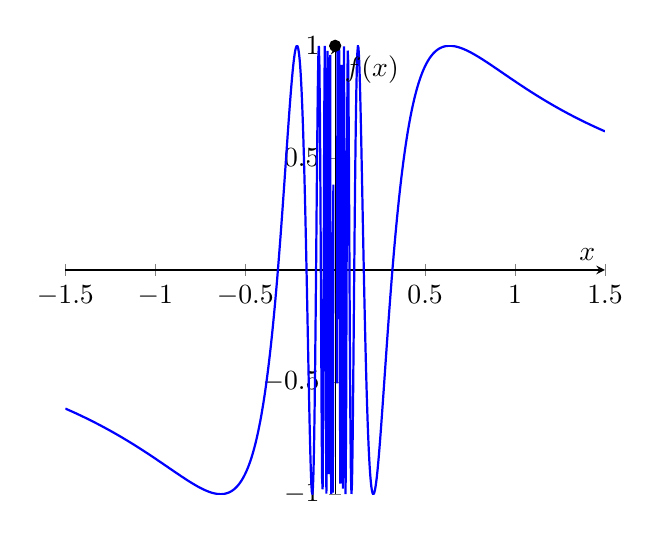
\begin{tikzpicture}
			\begin{axis}[
				axis lines = middle,
				xlabel = \( x \),
				ylabel = \( f(x) \),
				domain = -1.5:1.5,
				samples = 500,
				restrict y to domain=-2:2, % Limit y to make the oscillations visible
				]
				% Plot for x != 0 (sin(1/x))
				\addplot[blue, thick, domain=-1.5:-0.01] {sin(deg(1/x))};
				\addplot[blue, thick, domain=0.01:1.5] {sin(deg(1/x))};
				% Mark the point at x = 0 where f(x) = 1
				\addplot[mark=*, only marks, black] coordinates {(0, 1)};
			\end{axis}
		\end{tikzpicture}
		\caption{\en{Plot of \( f(x) = \sin(1/x) \) for \( x \neq 0 \)}}
	\end{figure}
\end{example}
\newpage
\begin{example}
	الدالة
	\[
	f(x) =
	\begin{cases}
		x\sin \dfrac{1}{x} & x\neq0 \\
		1 & x=0
	\end{cases}
	\]
	تمتلك عدم استمرارية قابلة للحذف لان
	 $f(0+) = f(0-) = 0$
	 و $f(0) = 1$ 
	 	\begin{figure}[H]
	 	\centering
	 	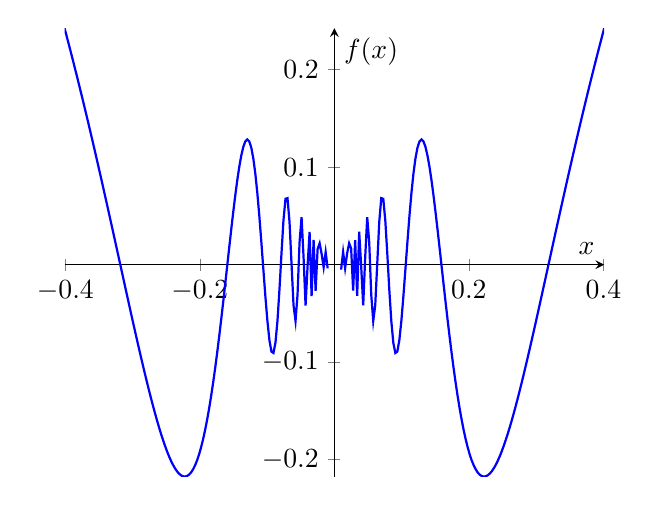
\begin{tikzpicture}
	 		\begin{axis}[
	 			axis lines = middle,
	 			xlabel = \( x \),
	 			ylabel = \( f(x) \),
	 			domain = -1.5:1.5,
	 			samples = 500,
	 			restrict y to domain=-2:0.25, % Limit y to make the oscillations visible
	 			]
	 			% Plot for x != 0 (sin(1/x))
	 			\addplot[blue, thick, domain=-1.5:-0.01] {x*sin(deg(1/x))};
	 			\addplot[blue, thick, domain=0.01:1.5] {x*sin(deg(1/x))};
	 			% Mark the point at x = 0 where f(x) = 1
	 			\addplot[mark=*, only marks, black] coordinates {(0, 1)};
	 		\end{axis}
	 	\end{tikzpicture}
	 	\caption{\en{Plot of \( f(x) =x \sin(1/x) \) for \( x \neq 0 \)}}
	 \end{figure}
\end{example}

\begin{example}
	الدالة $f(x) = \exp\left(\dfrac{1}{x}\right)$ تمتلك عدم استمرارية اساسية عند $x=0$ لأن الغايات
	\[
	\lim\limits_{x\to 0} \exp\left(\frac{1}{x}\right), \quad 	\lim\limits_{x\to 0^+} \exp\left(\frac{1}{x}\right), 
	\]
	غير موجودة ولكن 
	\[
		\lim\limits_{x\to 0^-} \exp\left(\frac{1}{x}\right) = 0
	\]
\end{example}

\newpage

\begin{example}
اوجد نقاط عدم الاستمرارية للدالة وصنفها
	\[
	f(x) =
	\begin{cases}
		\dfrac{x^2 - 4}{x -2} & x \neq 2 \\
		1 & x =2
	\end{cases}
	\]
\end{example}
\begin{solution}
 نلاحظ
	\[
	\lim\limits_{x\to 2} f(x) = \lim\limits_{x\to 2} \frac{(x-2)(x+2)}{x-2} = \lim\limits_{x\to 2} x+2 = 4
	\]
	ولكن $f(2) = 1$ اذن $x=2$ نقطة عدم استمرارية قابلة للحذف. وذلك بأعادة تعريف الدالة عند $x=2$ لتكون $f(2) = 4$.
	\end{solution}
	\begin{example}
		اوجد نقاط عدم الاستمرارية وصنفها
		\[
		f(x) = 
		\begin{cases}
			\dfrac{x^2 - 4x +3}{2x-2} & x > 1 \\
			3 & x=1\\
			\dfrac{x^2 - 1}{x-1} & x<1
		\end{cases}
		\]
	\end{example}
	\begin{solution}
		نوجد غاية اليمين عند $x=1$ 
		\[
		\lim\limits_{x\to 1^+} f(x) = \lim\limits_{x\to 1^+} \frac{(x-1)(x-3)}{2(x-1)} = \lim\limits_{x\to 1^+} \frac{x-3}{2} = -1
		\]
		بينما غاية اليسار
		\[
		\lim\limits_{x\to 1^-} f(x) = \lim\limits_{x\to 1^-} \frac{(x-1)(x+1)}{x-1} =\lim\limits_{x\to 1^-} x+1 =2
		\]
		ولكن $f(1)=3$. اذن $x=1$ نقطة عدم استمرارية غير قابلة للحذف لأنه لا يمكن اعادة تعريف الدالة عند $x=1$ لتكون الدالة مستمرة عند تلك النقطة وذلك لأن غاية اليمين لا تساوي غاية اليسار.
	\end{solution}

\newpage
\section[المشتقات عند الدوال غير المستمرة]{المشتقات عند الدوال غير المستمرة \cite{mathanalysis}}
لدراسة الدوال غير المستمرة في الاشتقاق. نقدم مفهوم المشتقة من اتجاه واحد والمشتقة اللا نهائية.
\begin{definition}[( المشتقة من اتجاه واحد )]
	لتكن $f$ دالة معرفة على الفترة المغلقة $[a, b]$ نقول ان $f$ تمتلك مشتقة يمينية عند $c$ اذا كانت الغاية 
	\[
	\lim\limits_{x\to c^+} \frac{f(x) - f(c)}{x-c}
	\]
	موجودة كقيمة نهائية او ان الغاية هي $+\infty$ او $-\infty$ و نرمز لها بالرمز $f_+'(x)$. المشتقة اليسارية تعرف بنفس الاسلوب
	\[
f_-'(c):=	\lim\limits_{x\to c^-} \frac{f(x) - f(c)}{x-c}
	\]
\end{definition}

\begin{example}
	لتكن الدالة $f(x) = |x|$، رأينا في المثال 1 - 3 - 1 ان الدالة لا تمتلك مشتقة عند  $x=0$ ولكن
	\[
f_+'(0) = \lim\limits_{x\to0^+} \frac{|x|}{x} = \lim\limits_{x\to0^+} \frac{x}{x} =1
\]
\[
f_-'(0) = \lim\limits_{x\to0^-} \frac{|x|}{x} = \lim\limits_{x\to0^-} \frac{-x}{x}=- 1
\]

\begin{figure}[H]
	\centering
	\begin{tikzpicture}
		\begin{axis}[
			axis lines = middle,
			xlabel = $x$,
			ylabel = {$f(x)$},
			xmin = -5, xmax = 5,
			ymin = 0, ymax = 5,
			samples = 100
			]
			\addplot[domain=-5:5,blue,thick] {abs(x)};
		\end{axis}
	\end{tikzpicture}
	\caption{$f(x) = |x|$}
\end{figure}
\newpage
\end{example}

\begin{example}
	لتكن 
\[
f(x)=
\begin{cases}
	\dfrac{1}{2}x^2 + 1 & x\leq 2 \\
	x+2 & x>2
\end{cases}
\]	
الدالة غير مستمرة عند $x=2$ لأن 
\[
f(2^+) = 4 \neq 2 = f(2^-)
\]
ولكن 
\begin{align*}
	f_+'(2) &= \lim\limits_{x\to 2^+} \frac{f(x) - f(2)}{x-2} \\
	&= \lim\limits_{x\to 2^+} \frac{x+2-3}{x-2} \\
	&= \lim\limits_{x\to2^+} \frac{x-1}{x-2} = -\infty
\end{align*}
و
\begin{align*}
	f_-'(2) &= \lim\limits_{x\to 2^-} \frac{\dfrac{1}{2} x^2 +1 -3}{x-2}\\
	&= \lim\limits_{x\to 2^-} \frac{\dfrac{1}{2}(x^2-4)}{x-2} \\
	&= \lim\limits_{x\to 2^-} \frac{\dfrac{1}{2}(x-2)(x+2)}{x-2}\\
	&= \lim\limits_{x\to 2^-} \frac{1}{2}(x+2)\\
	&= 2
\end{align*}
\begin{figure}[H]
		\centering
		\begin{tikzpicture}
			\begin{axis}[
				axis lines = middle,
				xlabel = $x$,
				ylabel = {$f(x)$},
				xmin = -5, xmax = 5,
				ymin = -2, ymax = 10,
				samples = 100
				]
				\addplot[domain=-5:2,blue,thick] {0.5*x^2 + 1};
				\addplot[domain=2:5,red,thick] {x + 2};
			\end{axis}
		\end{tikzpicture}
		\caption{\en{Plot of \(f(x)\)}}
\end{figure}
\end{example}

\section[الاستمرارية بالأجزاء]{الاستمرارية بالاجزاء \cite{ode1}}

\begin{definition}[( الاستمرارية بالأجزاء )]
	نقول ان الدالة $f(x)$ مستمرة بالاجزاء على الفترة المغلقة $[a, b]$ اذا كانت مستمرة عند عدد منتهِ من نقاط عدم الاستمرارية القفزية
\end{definition}

\begin{example}
	الدالة 
	\[
	f(x) =
	\begin{cases}
		x^3  & 0\leq x\leq 1 \\
		1-x & 1\leq x \leq 2\\
		1 & 2\leq x \leq 3
	\end{cases}
	\]
\end{example}

\begin{note}
	ليس مطلوب ان تكون الدالة $f(x)$ معرفة عند نقاط عدم الاستمرارية القفزية. لنفر	ض ان $a_1, \dots, a_n$ مواقع عد الاستمرارية القفزية للدالة $f$ في الفترة $[a, b]$ ونفرض ان $a_i < a_{i+1}$ لكل $i$، على الفترة $(a_i, a_{i+1})$ يمكننا جعل $f(x)$ دالة مستمرة على الفترة المغلقة $[a_i, a_{i+1}]$ من خلال تعريف
	\[
	f(a_i) = \lim\limits_{x\to a_i^+}f(x), \quad f(a_{i+1}) = \lim\limits_{x\to a_{i+1}^-} f(x)
	\]
	ولأن الدالة المستمرة على الفترة المغلقة تكون مقيدة لدينا المبرهنة التالية
\end{note}

\begin{theorem}
	اذا كانت $f(x)$ دالة مستمرة بالاجزاء على الفترة $[a, b]$ فإن $f(x)$ تكون مقيدة.
\end{theorem}

\section[تكامل الدوال المستمرة بالاجزاء]{تكامل الدوال المستمرة بالاجزاء \cite{ode2}}

\begin{definition}
	اذا كانت $f(x)$ مستمرة بالاجزاء على الفترة $[a , b]$ ونقاط عدم الاستمرارية عند \\$a_1<a_2<\cdots<a_k$، لتكن $a=a_0, b=a_{k+1}$. كما لاحظنا فإننا من الممكن جعل الدالة $f$ مستمرة على $[a_i, a_{i+1}]$ وبالتالي من الممكن تعريف التكامل المحدد للدالة $f$ على الفترة $[a, b]$ كما يلي
	\[
	\int_{a}^{b} f(x) \, dx = \int_{a_0}^{a_1} f(x)\, dx + \int_{a_1}^{a_2} f(x) \, dx + \cdots + \int_{a_k}^{a_{k+1}} f(x) \, dx
	\]
\end{definition}

\begin{example}
	نجد التكامل للدالة $f(x)$ المعرفة بالشكل
	\[
	f(x) = 
	\begin{cases}
		1 & 0\leq x< 1 \\
		0 & 1\leq x < \infty
	\end{cases}
	\]
	على الفترة $[0, t]$ حيث $t\in [0,\infty)$. لدينا احتمالان هنا:\\
	1. اذا كان $t\in [0,1)$ فإن 
	\[
	\int_{0}^{t} f(x) \, dx = \int_{0}^{t} 1 \, dx = t
	\]
	2. اذا كان $t\in [1, \infty)$ فإن 
	\begin{align*}
		\int_{0}^{t}f(x) \, dx &=\int_{0}^{1}f(x) \, dx + \int_{1}^{t} f(x) \, dx\\
		&= \int_{0}^{1}1 \, dx + \int_{1}^{t} 0 \, dx\\
		&= 1
	\end{align*}
	اذن 
	\[
	\int_{0}^{t}f(x)\, dx = 
	\begin{cases}
		t & 0\leq t<1 \\
		1 & 1 \leq t < \infty
	\end{cases}
	\]
\end{example}

\begin{english}
	\begin{figure}[H]
	\centering
	\begin{subfigure}{0.45\textwidth}
		\centering
			\begin{tikzpicture}
			\begin{axis}[
				axis lines=middle,
				xlabel={$x$},
				ylabel={$y$},
				ymin=-0.2, ymax=3,
				xmin=-0.2, xmax=3,
				domain=0:3,
				samples=100
				]
				
				\addplot[blue, thick] coordinates {(1,0)  (3,0)};
				\addplot[blue, thick] coordinates {(0,1)  (1,1)};
				
				\addplot[blue, only marks, mark=*] coordinates {(1,0)};
				\addplot[blue, only marks, mark=o] coordinates {(1,1)};
			\end{axis}
		\end{tikzpicture}
		\caption{plot of $f(x)$}
	\end{subfigure}
	\hfill
	\begin{subfigure}{0.45\textwidth}
		\centering
			\begin{tikzpicture}
			\begin{axis}[
				axis lines=middle,
				xlabel={$x$},
				ylabel={$y$},
				ymin=-0.2, ymax=3,
				xmin=-0.2, xmax=3,
				domain=0:3,
				samples=100
				]
				
				\addplot[red, thick, domain=0:1] {x};
				\addplot[red, thick] coordinates {(3,1)  (1,1)};
				
				\addplot[red, only marks, mark=*] coordinates {(1,1)};
			\end{axis}
		\end{tikzpicture}
		\caption{plot of $\int_{0}^{t} f(x)\, dx$}
	\end{subfigure}
\end{figure}
\end{english}

\begin{note}
	نلاحظ ان الدالة $\int_{0}^{x} f(u)\, du$ مستمرة على الرغم من كون الدالة $f(x)$ دالة غير مستمرة. وهذا دائماً صحيح مادام ان الدالة $f(x)$ تمتلك عدد منتهِ من نقاط عدم الاستمرارية القفزية.
\end{note}

\begin{theorem}
	اذا كانت $f(x)$ دالة مستمرة  بالاجزاء على الفترة $[a, b]$ وأن $c,t\in [a,b]$. فإن التكامل
	 $\int_{c}^{t} f(x)\, dx$
	 دالة مستمرة للمتغير $t$. 
\end{theorem}
\noindent
\textbf{البرهان}\\
\noindent
لتكن
\[
F(t) = \int_{c}^{t} f(x)\, dx
\]
بما ان $f(x)$ دالة مستمرة بالاجزاء على $[a, b]$ اذن هي مقيدة. لنفرض $|f(x)| \leq B$ لبعض $B>0 $. نفرض $\epsilon > 0 $. فإن 
\[
|F(t+\epsilon) - F(t)| \leq \int_{t}^{t+\epsilon} |f(x)|\,dx \leq \int_{t}^{t+\epsilon} B\, dx=B\epsilon
\]
اذن 
$\lim\limits_{\epsilon\to0} F(t+\epsilon) = F(t)$ ومنه $F(t^+) = F(t)$ بطريقة مماثلة $F(t^-) =F(t)$ وهذا يثبت استمرارية $F(t)$


\section[التقارب للدوال غير المستمرة]{التقارب للدوال غير المستمرة \cite{realanal}}
سوف نناقش بعض الامثلة لدوال مستمرة تقترب بشكل نقطي الى دالة غير مستمرة. ومثال على متتابعة على من الدوال غير المستمرة تقترب نقطياً الى دالة مستمرة

\begin{example}
	لتكن لدينا المتتابعة من الدوال المستمرة $f_n(x) = x^n$. نلاحظ اذا كان $x=1$ فإن
\[
\lim\limits_{n\to \infty} f_n(1) = \lim\limits_{n\to \infty} 1 =1
\]
	بينما اذا كان $0<x<1$ فإن 
	\[
	\lim\limits_{n\to \infty} x^n = 0
	\]
\end{example} 
اي ان 
\[
\lim\limits_{n\to \infty} f_n(x) = 
\begin{cases}
	0 & 0 <x< 1  \\
	1 & x=1
\end{cases}
\]
وهذه الدالة غير مستمرة عند $x=1$.

\begin{example}
	لنأخذ المتتابعة من الدوال غير المستمرة 
	\[
	f_n(x) = 
	\begin{cases}
		\dfrac{1}{n} & x\notin \Q \\[10pt]
		0 & x\in \Q
	\end{cases}
	\]
	هذه الدالة غير مستمرة لكل $x\in\R$ ولكن نلاحظ ان اذا كان $x\in\Q$ فإن 
	$f_n(x) = 0 \to 0$
	و اذا كان $x\notin \Q$ فإن 
	\begin{english}
		\[
	f_n(x) = \frac{1}{n} \to 0 \quad \text{as $x\to \infty$}
	\]
	\end{english}
	اي ان المتتابعة تتقارب بشكل نقطي الى الدالة $f(x) = 0 $ بشكل نقطي. وهي دالة مستمرة.
\end{example}

	
	\chapter*{الاستنتاجات}
\addcontentsline{toc}{chapter*}{الاستنتاجات}
من خلال دراسة طريقة متسلسلات القوى لحل المعادلات التفاضلية الاعتيادية، توصلنا إلى عدة استنتاجات مهمة تتعلق بكفاءة هذه الطريقة ودورها في إيجاد الحلول في الحالات التي يصعب فيها استخدام الطرق التحليلية الأخرى. يمكن تلخيص أهم هذه الاستنتاجات كما يلي:
\begin{enumerate}
	\item قابلية التطبيق على معادلات متنوعة: تُعد طريقة متسلسلات القوى أداة قوية لحل المعادلات التفاضلية التي تحتوي على معاملات متغيرة، والتي قد لا تكون قابلة للحل باستخدام الطرق التقليدية مثل الفصل أو التكامل المباشر.
	\item  تمثيل الحل بشكل دقيق: من خلال التعبير عن الحل كسلسلة لا نهائية من الحدود، يمكن الحصول على تمثيل دقيق للحل في منطقة التقارب، مما يسهل إيجاد تقديرات عددية محسنة عند الحاجة.
\end{enumerate}



	
	\begin{thebibliography}{9}
		\addcontentsline{toc}{chapter*}{المصادر}
		\bibitem{key1}
		\begin{english}
		James C. Robinson, \textit{An Introduction to Ordinary Differential Equations}, Cambridge University Press, New York, 2004.
		
		\bibitem{key2}
		M. Tenenbaum, H. Pollard, \textit{Ordinary Differential Equations}, Dover Publications, 1985.
		
		\bibitem{key3}
		S. N. Elaydi, \textit{An Introduction to Difference Equations}, 3rd ed., Springer, 2005.
		
		\bibitem{key4}
		E. A. Coddington, N. Levinson, \textit{Theory of Differential Equations}, McGraw-Hill, 1955.
		\end{english}
	\end{thebibliography}

\end{document}